% !TeX root = ../main.tex
% Add the above to each chapter to make compiling the PDF easier in some editors.

\chapter{Building Flows in Weight-Space}\label{chapter:method}

We now bring the preceding background together and describe how we can build flows in weight-space. We propose three alternative formulations based on how the scaling symmetries are handled: first a Euclidean flow defined in weight-space directly, and then the Normalized and Geometric flows with the weights normalized to remove the scaling symmetries, differing on whether the vector field is also defined in Euclidean space (Normalized flow) or on the manifold of normalized weights (Geometric flow). We conclude by describing by how we train and sample from our flows. 

\section{Training With and Without Samples}

Although simulation-free methods to train generative models with score/flow-matching objectives only given access to an unnormalized density function exist \citep{akhound-sadeghIteratedDenoisingEnergy2024}, we train our models on samples obtained using typical gradient-based optimization of neural networks. This is an easier setup and allows us to measure the impact of various design choices more clearly, and also potentially benefit from publicly available datasets of neural network weights \citep{schurholtModelZoosDataset2022,peeblesLearningLearnGenerative2022}. Thus, for each training task, we independently train a number of neural networks and intermittently save the weights along each SGD trajectory, discarding the initial steps based on validation loss, to train our flow models with. 

\section{Flows on Different Geometries}

\begin{figure}[h!]
    \centering
    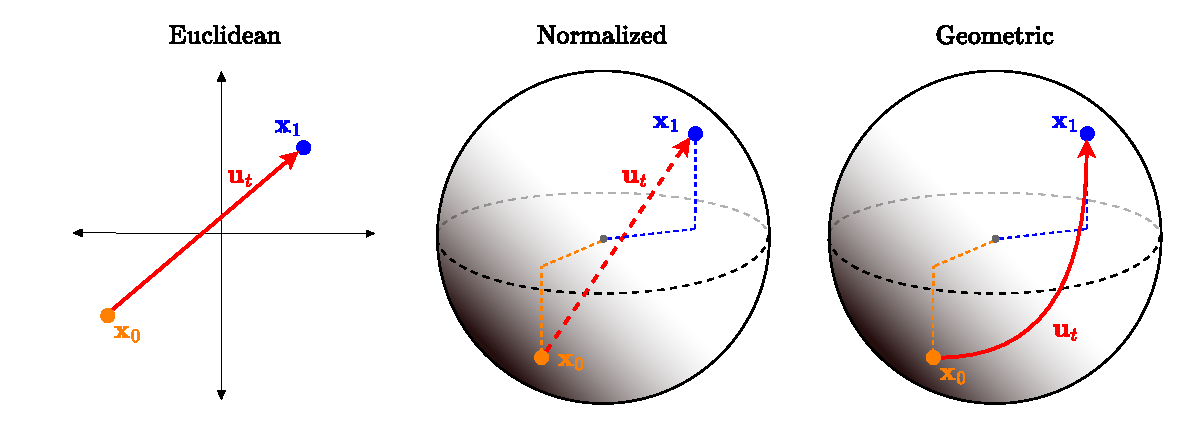
\includegraphics[width=\textwidth]{figures/flow_types.drawio.pdf}
    \caption{\label{fig:flow_types}\textbf{Flows with different geometric structures.} \textit{Left:} Euclidean flow defined over in weight-space without modifying the weights. \textit{Center:} Normalized flow after removing scaling symmetries, with the vector field defined as in Euclidean space. \textit{Right:} Geometric flow, with the vector field defined over the particular geometry as well.}
\end{figure}

The first step in designing a flow is to determine the space our data lies in. We propose three different approaches with different geometric properties, illustrated in Figure \ref{fig:flow_types}: first a Euclidean flow operating directly over the trained weights, and then two different methods operating with the normalized weights as described in Section \ref{section:geometry_of_nns} following the process of \citep{pittorinoDeepNetworksToroids2022}. The last two methods further differ on whether the vector space is also over these normalized weights or not. 

\subsection{Euclidean Flow}

Our first method we call the Euclidean flow is defined in Euclidean space, and the trained weights are used directly, without any transformations except alignment to a common reference.  Following the presentation in Section \ref{section:flow_matching}, we define the ground truth vector field as $x_1 - x_0$. Such a flow can be straightforwardly applied to any neural network, but ignores the scaling symmetries resulting from activations such as ReLU. 

\begin{figure}[t!]
    \centering
    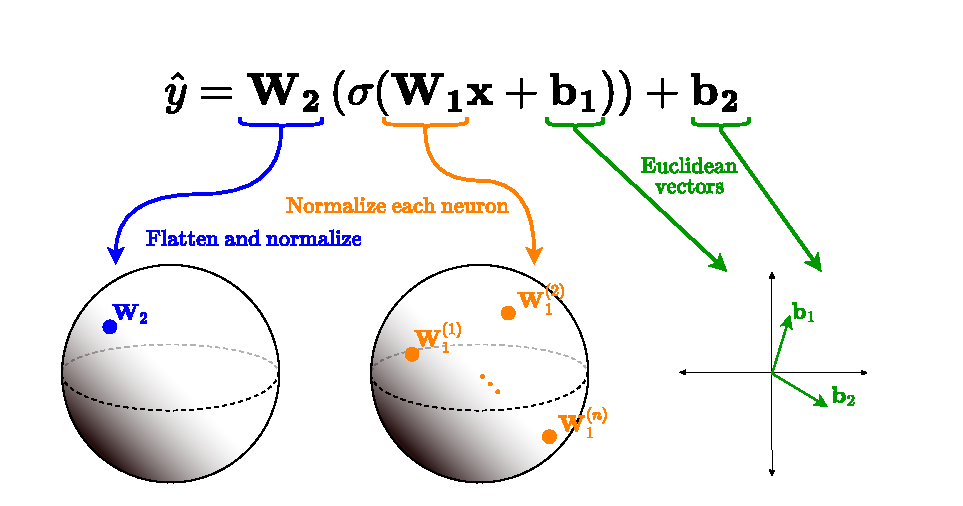
\includegraphics[width=\textwidth]{figures/canonicalization.drawio.pdf}
    \caption{\label{fig:canonicalization}\textbf{Removing scaling symmetries from ReLU networks.} Each intermediate neuron lies on a unit hypersphere, as well as the last layer as a whole. Bias vectors are also rescaled but remain Euclidean vectors.}
\end{figure}


\subsection{Normalized Flow}

A simple modification to the Euclidean flow above is to first apply the normalization procedure of \citep{pittorinoDeepNetworksToroids2022} as shown in Figure \ref{fig:canonicalization}. To recap for ReLU networks, we normalize the incoming weight vector and bias of each intermediate neuron, and scale the outgoing weight vector up by the same factor to preserve the function being computed by the neural network. Since there is no such symmetry for the last layer, we normalize the entire last layer weights for a classification as that would preserve the output class. We leave the last layer unchanged for regression tasks. 

This procedure embeds neural network weights in a product geometry. Each intermediate neuron, and the last layer in its entirety, now lie on unit hyperspheres of different dimensions. The bias vectors have no such structure and we still treat them as Euclidean vectors. Our Normalized flow works with source and target distributions on this product geometry, but the vector field is still defined in Euclidean space; i.e. inside the hyperspheres for neurons and in Euclidean space for biases. This is an intermediate step between the previous Euclidean flow and the Geometric flow we will describe next. 

\subsection{Geometric Flow}

Since hypspheres are Riemannian manifolds, we can model vector fields over them using the framework of Riemannian flow matching \citep{chenRiemannianFlowMatching2023} (Section \ref{sec:riemannian_fm}). For the bias vectors in Euclidean space, we again define $u_t := x_1 - x_0$ and $x_t = t x_1 + (1-t) x_0$. For intermediate neurons and the last layer on different hyperspheres, we have $x_t = \exp_{x_0}(t \log_{x_0}x_1)$ and $u_t = \log_{x_t}(x_1) / (1-t)$. This formulation, while computationally more expensive, has the added potential benefit that all inputs including the intermediate points $x_t$ to our model will lie on this particular geometry, reducing the effective dimensionality of the problem. 

While we focus only on ReLU networks, this geometric formulation can be extended to other nonlinearities as they also induce different kinds of scaling symmetries \citep{godfreySymmetriesDeepLearning2022}. 

\section{Model Architecture}

For each of our three flows, we model the vector field using a Relational Transformer with edge updates \citep{diaoRelationalAttentionGeneralizing2023,kofinasGraphNeuralNetworks2024}. For an MLP as the base model, each edge in the graph corresponds to a single weight, and nodes to individual bias values. We project each node and edge feature to $d_E$ dimensions using an MLP, and run a number of node/edge update steps before projecting the final node/edge states back to one dimension using an MLP. To distinguish nodes at different layers, we add layer-specific learned positional embeddings to edge features. 

\section{Training}

We train our models using the conditional flow matching \textbf{objective} (Equation \ref{eq:cfm_objective}), but rather than predict the velocity $u_t$, we predict the target point $x_1$ and compute the velocity during integration the using initial point $x_0$ and intermediate point $x_t$. This simplifies training as the error in weight-space is more informative, and we can constrain the inputs to the particular geometry for the Normalized and Geometric flows. 

\begin{wrapfigure}{r}{0.4\textwidth}
    \centering
        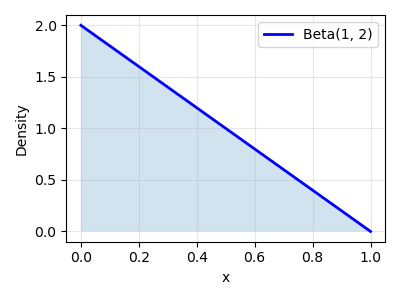
\includegraphics[width=\linewidth]{figures/beta.png}
    \caption{\label{fig:beta}\textbf{PDF of $\text{Beta}(1,2)$.} We sample $t\sim \text{Beta}(1,2)$ rather than uniformly when training our flow model.}
\end{wrapfigure}


As \textbf{prior} distributions $p_0$, we use isotropic Gaussians of different variances, ensuring that the prior distribution is the same as the distribution used to initialize the weights while training the base model, although this is not a strict requirement and our flow models can be trained with arbitrary priors. We also experiment with independent and mini-batch optimal transport \textbf{couplings}, although especially in high-dimensions the bias induced by the mini-batch approximation to optimal transport can be significant \citep{fatrasMinibatchOptimalTransport2021}. 

As another modification over the standard flow matching framework, we sample \textbf{time} $t \in (0,1)$  during training not uniformly, but following $\text{Beta}(1,2)$ (Figure \ref{fig:beta}). Since $x_t$ with smaller $t$ are further away from $x_1$, estimation error increases for smaller time values. Sampling $t \sim \text{Beta}(1,2)$ results in a larger number of parameter updates for smaller $t$ relative to larger $t$, which is a more effective distribution of the computational budget since the predictions for smaller $t$ converge in fewer updates. Importantly, sampling $t \sim \text{Beta}(1,2)$ does not modify or bias the training process, since a prediction at a certain time is independent of the model performance at other times. 

\section{Sampling}

To sample from our flow models, we solve the ODE (Equation \ref{eq:ode}) using an Euler solver with step sizes ranging from 10 to 250 depending on the complexity of the task, although higher-order solvers can also be used without any modification to the rest of the setup. We also experiment with \textbf{stochastic sampling} by adding noise before computing Euler updates, on the entire trajectory or a subset of it \citep{karrasElucidatingDesignSpace}. 

\subsection{Guidance}

We can also guide the sampling process with loss gradients from the base task \citep{wangProteinConformationGeneration2024,kulyteImprovingAntibodyDesign2024,yuForceGuidedBridgeMatching2024a}, so that for base model $f$ and velocity model $v_\theta$ Euler updates take the form 
\begin{equation}
    x_{t + \Delta t} = x_t + \left( v_\theta(t, x_t) + \lambda \nabla_{x_t}\mathcal{L}(f, x_t) \right) \Delta t
\end{equation}
where $\mathcal{L}(f, x_t)$ is computed with training data points from the base task (note that $x_t$ are the model parameters), and $\lambda$ is a coefficient controlling the strength of this guidance. If the task loss $\mathcal{L}$ is computed with mini-batches, this guidance also adds an implicit stochasticity to each step of the sampling process. 

